\documentclass[../main.tex]{subfiles}

\begin{document}

\section{Riemannův integrál ve více proměnných}

\begin{figure}[h]
	\centering
	\subfloat[Funkce ve více proměnných]{{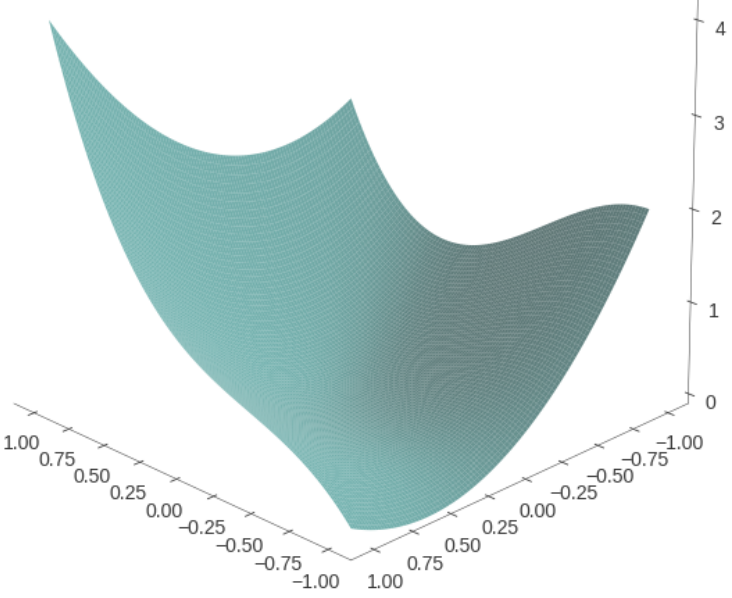
\includegraphics[width=6cm]{09-funkce} }}%
	\hspace{4em}
	\subfloat[Horní součet funkce]{{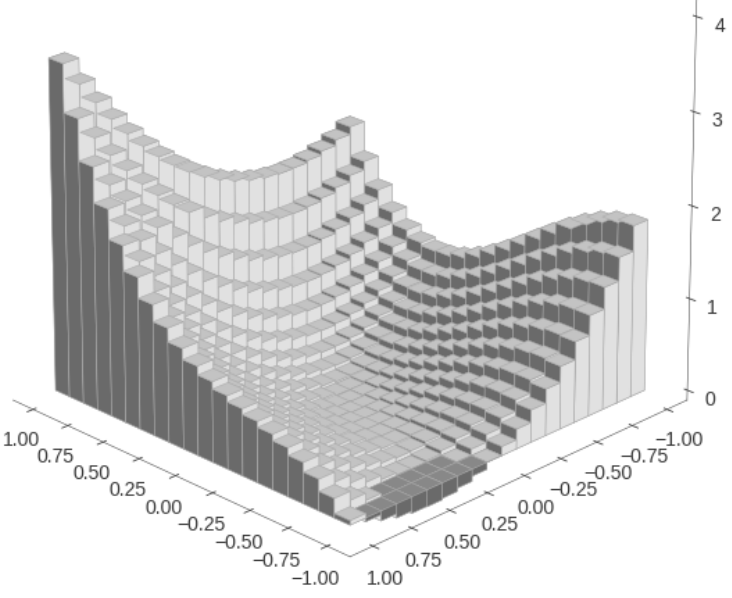
\includegraphics[width=6cm]{09-integral} }}%
	\caption{Geometrický význam Riemannova integrálů ve více proměnných.}
\end{figure}

\subsection{Definice}

\begin{definitionnodot}[$n$-rozměrný kompaktní interval]
	 (v $\mathbb{E}_n$) je 
	\[J = \left<a_1,b_1\right> \times \cdot \cdot \cdot \times \left<a_n,b_n\right>\]
\end{definitionnodot}

\begin{definitionnodot}[Rozdělení intervalu]
	$J$ je posloupnost rozdělení $P = (P^1,...,P^n)$:
	\[P^j : a_j = t_{j,0} < t_{j,1} < \cdot \cdot \cdot < t_{j,n_j-1} < t_{j,n_j} = b_j\]
\end{definitionnodot}

\begin{definition}[Cihly]
	Intervalům
	\[\left<t_{1,i_1},t_{1,i_1+1}\right> \times \cdot \cdot \cdot \times \left<t_{n,i_n},t_{n,i_n+1}\right>\]
	říkáme \textbf{cihly rozdělení $P$} a $$\mathcal{B}(P)$$ je množina všech cihel rozdělení $P$. Je to skoro disjunktní rozdělení intervalu $J$.
	Různé cihly z $\mathcal{B}(P)$ se totiž setkávají jen v podmnožinách okrajů, tedy v množinách objemu 0, díky čemuž platí:
	\[\textbf{vol}(J) = \sum \{\textbf{vol}(B) : B \in \mathcal{B}(J)\}.\]
\end{definition}

\begin{definitionnodot}[Průměr (diametr)]
	intervalu $J = \left<r_1,s_1\right> \times \cdot \cdot \cdot \times \left<r_n,s_n\right>$ je
	\[\textbf{diam}(J) = \max_i (s_i - r_i)\]
\end{definitionnodot}

\begin{definitionnodot}[Jemnost]
	rozdělení $P$ je 
	\[\mu(P) = \max \{\textbf{diam}(B) : B \in \mathcal{B}(P)\}\]
\end{definitionnodot}

\begin{definition}[Zjemnění]
	Rozdělení $Q = (Q^1,...Q^n) $ zjemňuje rozdělení $P = (P^1,...,P^n)$ jestliže každé $Q^j$ zjemňuje $P^j$.
	Vytváří/indukuje tak rozdělení $Q_B\ \forall B \in \mathcal{B}(P)$ a jistě platí
	\[\mathcal{B}(Q) = \bigcup \{\mathcal{B}(Q_B) : B \in \mathcal{B}(P)\}.\]
\end{definition}

\begin{observation}
	Každá dvě rozdělení $P,Q$ $n$-rozměrného kompaktního intervalu $J$ mají společné zjemnění.
\end{observation}

\begin{definition}[„Supremum/infimum“ na kompaktním intervalu]
	Je dána omezená $f: J \rightarrow \mathbb{R}$ na $n$-rozměrném kompaktním intervalu $J$ a $B \subseteq J$ je 
	$n$-rozměrný kompaktní podinterval intervalu $J$. Položme
	\[m(f,B) = \inf\{f(\textbf{x}) : \textbf{x} \in B\} \qquad \text{a} \qquad M(f,B) = \sup\{f(\textbf{x}) : \textbf{x} \in B\}.\]
\end{definition}

\begin{observation}
	$m(f,B) \leq M(f,B)$ a je-li $C \subseteq B$, pak 
	\[m(f,C) \geq m(f,B) \qquad \text{ a } \qquad M(f,C) \leq M(f,B).\]
\end{observation}

\begin{definition}[Horní/dolní součty]
	Pro rozdělení $P$ intervalu $J$ a omezenou funkci $f : J \rightarrow \mathbb{R}$ definujeme 
	\[s_J(f,P) = \sum \{m(f,B) \cdot \textbf{vol}(B) : B \in \mathcal{B}(P)\},\]
	\[S_J(f,P) = \sum \{M(f,B) \cdot \textbf{vol}(B) : B \in \mathcal{B}(P)\}.\]
\end{definition}

\begin{observation}[obecné]
	$f: X \rightarrow \mathbb{R}$ je omezená, $X = \bigcup X_i$ a $X_i = \bigcup X_{ij}$ jsou konečná skoro disjunktní sjednocení. Nechť dále (a analogicky pro $m$ infima):
	\[M_i = \sup\{f(x) : x \in X_i\},\]
	\[M_{ij} = \sup\{f(x) : x \in X_{ij}\}\]
	Triviálně $M_{ij} \leq M_i$ ( $M_i$ je horní mez množiny $\{f(x) : x \in X_{ij}\}$), tedy:
	$$
	\begin{aligned}
		\sum M_i \textbf{vol}(X_i) &= \sum_i M_i \sum_j \textbf{vol}(X_{ij}) \\
	  &= \sum_{ij}M_i \textbf{vol}(X_{ij}) \\
		&\geq \sum_{ij} M_{ij} \textbf{vol}(X_{ij})
	\end{aligned}
	$$
\end{observation}

\begin{lemma}
	Nechť $Q$ zjemňuje $P$. Potom
	\begin{center}
	    \begin{tabular}{c c c}
	        $s(f,Q) \geq s(f,P)$ & a & $S(f,Q) \leq S(f,P)$
	    \end{tabular}
	\end{center}
\end{lemma}

\begin{proof}
	Použijeme předchozí pozorování pro $\{X_i\ |\ i\} = \mathcal{B}(P)$, $\{X_{ij}\ |\ j\} = \mathcal{B}(Q_B)$ a samozřejmě
	i pro $\{X_{ij}\ |\ ij\} = \mathcal{B}(Q).$
\end{proof}

\begin{lemma}
	Pro libovolná dvě rozdělení $P,Q$ intervalu $J$ máme $s(f,P) \leq S(f,Q)$.
\end{lemma}

\begin{proof}
	Jelikož je triviálně $s(f,P) \leq S(f,P),$ použitím společného zjemnění $R$ rozdělení $P,Q$ dostaneme
	\[s(f,P) \leq s(f,R) \leq S(f,R) \leq S(f,Q).\]
\end{proof}

\begin{definition}[(Horní/dolní) Riemannův integrál]
	Množiny $\{s(f,P) \mid P \text{ rozdělení}\}$ a $\{S(f,P) \mid P \text{ rozdělení}\}$ jsou shora/zdola omezené (předchozí tvrzení) a můžeme definovat dolní/horní Riemannův integrál funkce $f$ přes $J$ jako
	\[\underline{\int}_J f(\textbf{x})d\textbf{x} = \sup\{s(f,P) \mid P \text{ rozdělení}\} \qquad \text{a} \qquad
	\overline{\int}_J f(\textbf{x})d\textbf{x} = \inf\{S(f,P) \mid P \text{ rozdělení}\}.\]
	Jsou-li si rovny, máme Riemannův integrál funkce $f$ přes $J$, značíme\footnote{Někdy se také značí jako \(\int_J f(x_1,...,x_n)dx_1,...x_n \text{ nebo } \int_J f(x_1,...,x_n)dx_1 dx_2\cdot \cdot \cdot dx_n\)}.
	$$\int_J f(\textbf{x})d\textbf{x} \quad \text{nebo prostě} \quad \int_J f $$
\end{definition}

%%%%%%%%%%%%%%%%%%%%%%%%%%%%%%%%%%%%%%%%%%%%%%%%%%%%%%%%%%%%%%%%%%%%%%%%%%%%%%%%%%%%%%%%%%%%%%%%%%%%%%%%%
\subsection{Existence}
\begin{theorem}[Kritérium existence Riemannova integrálu]
	Riemannův integrál $\int_{J} f(\mathbf{x}) \,d\mathbf{x}$ existuje právě když
	$\forall \varepsilon > 0$ existuje rozdělení $P$ takové, že
	\[ S_J(f,P) - s_J(f,P) < \varepsilon \]
\end{theorem}

\begin{proof}
	Nerovnost dává \[ S_J(f,P) < \varepsilon + s_J(f,P) \]
	z toho dostaneme
	\[ \overline{\int} \leq S_J(f,P) \leq \varepsilon + s_J(f,P) \leq \varepsilon + \underline{\int} \leq
	\varepsilon + \overline{\int}\]
	pro libovolně malé $\varepsilon$.
\end{proof}

%%%%%%%%%%%%%%%%%%%%%%%%%%%%%%%%%%%%%%%%%%%%%%%%%%%%%%%%%%%%%%%%%%%%%%%%%%%%%%%%%%%%%%%%%%%%%%%%%%%%%%%%%
\subsection{Riemannův integrál pro spojité funkce}
\begin{theorem}[Riemannův integrál pro spojité funkce]
	Každá spojitá funkce $f: J \to \mathbb{R}$ na $n$-rozměrném kompaktním intervalu má Riemannův integrál
	$\int_{J}f$.
\end{theorem}

\begin{proof}
	V $\mathbb{E}_n$ budeme používat metriku $\sigma$ definovanou předpisem
	\[ \sigma (\mathbf{x}, \mathbf{y}) = \max_{i} |x_i - y_i| \]
	Jelikož je $f$ stejnoměrně spojitá, můžeme pro $\varepsilon > 0$ zvolit $\delta > 0$ takové, že
	\[ \sigma (\mathbf{x}, \mathbf{y}) < \delta \quad \Rightarrow \quad
	|f(\mathbf{x}) - f(\mathbf{y})| < \frac{\varepsilon}{\textrm{vol}(J)} \]
	Připomeňme si jemnost $\mu (P)$. Je-li $\mu (P) < \delta$, pak je $\textrm{diam}(B) < \delta$ pro všechny
	$ B \in \mathcal{B}(P) $ a tedy
	\begin{align*}
			M(f, B) - m(f, B) &= \sup\{ f(\mathbf{x}) \mid \mathbf{x} \in B \} -
			\inf\{ f(\mathbf{x}) \mid \mathbf{x} \in B\}\leq\\
			&\leq \sup\{ |f(\mathbf{x}) - f(\mathbf{y})|: \mathbf{x}, \mathbf{y} \in B \}
			= \frac{\varepsilon}{\textrm{vol}(J)}
	\end{align*}
	takže
	\begin{align*}
			S(f,P) - s(f,P) &= \sum \{ (M(f,B) - m(f,B))\cdot \textrm{vol}(B) \mid B\in \mathcal{B}(P) \}\leq\\
			&\leq \frac{\varepsilon}{\textrm{vol}(J)}\sum \{ \textrm{vol}(B) \mid B\in \mathcal{B}(P) \}
			= \frac{\varepsilon}{\textrm{vol}(J)}\textrm{vol}(J) = \varepsilon
	\end{align*}
\end{proof}

%%%%%%%%%%%%%%%%%%%%%%%%%%%%%%%%%%%%%%%%%%%%%%%%%%%%%%%%%%%%%%%%%%%%%%%%%%%%%%%%%%%%%%%%%%%%%%%%%%%%%%%%%
\subsection{Fubiniova věta}
\begin{theorem}[Fubiniova věta]
	Vezměme součin $J = J' \times J'' \subseteq \mathbb{E}_{m+n}$ intervalů $J' \subseteq \mathbb{E}_m$,
	$J'' \subseteq \mathbb{E}_n$. Nechť existuje
	\[ \int_{J} f(\mathbf{x}, \mathbf{y}) \,d\mathbf{xy} \]
	a nechť pro každé $\mathbf{x} \in J'$, resp. $\mathbf{y} \in J''$, existuje
	\[ \int_{J'} f(\mathbf{x}, \mathbf{y}) \,d\mathbf{x} \qquad \text{a} \qquad \int_{J''} f(\mathbf{x}, \mathbf{y}) \,d\mathbf{y} \]
	Potom je
	\[ \int_J f(\mathbf{x}, \mathbf{y}) \,d\mathbf{xy} =
	\int_{J'} \left( \int_{J''} f(\mathbf{x}, \mathbf{y}) \,d\mathbf{y} \right) \,d\mathbf{x} = 
	\int_{J''} \left( \int_{J'} f(\mathbf{x}, \mathbf{y}) \,d\mathbf{x} \right) \,d\mathbf{y}\]
\end{theorem}

\begin{example}
	Ve dvou proměnných
	\[ \int_{J} f = \int_{a_1}^{b_1} \left( \int_{a_2}^{b_2} f(x,y) \,dy \right) \,dx \]
	Ve třech proměnných
	\[ \int_{J} f =
	\int_{a_1}^{b_1} \left(
	\int_{a_2}^{b_2} \left(
	\int_{a_3}^{b_3} f(x_1, x_2, x_3) \,dx_3 \right) \,dx_2 \right) \,dx_1 \]
	Obecně
	\[ \int_{J} f =
	\int_{a_1}^{b_1} \left(
	\int_{a_2}^{b_2} \left(
	\dots \left(
	\int_{a_n}^{b_n} f(x_1, x_2, ..., x_n) \,dx_n \right) \dots \right) \,dx_2 \right) \,dx_1 \]
\end{example}

\begin{proof}
	Položme
	\[ F(\mathbf{x}) = \int_{J''} f(\mathbf{x}, \mathbf{y}) \,d\mathbf{y} \]
	Dokážeme, že $\int_{J'} F$ existuje a že
	\[ \int_{J} f = \int_{J'} F \]
	Zvolme rozdělení $P$ intervalu $J$ tak, aby
	\[ \int f - \varepsilon \leq s(f,P) \leq S(f,P) \leq \int f + \varepsilon \]
	Toto rozdělení je tvořeno rozděleními $P'$ intervalu $J'$ a $P''$ intervalu $J''$. Máme
	\[ \mathcal{B}(P) = \{ B' \times B'' \mid B' \in \mathcal{B}(P'), B'' \in \mathcal{B}(P'') \} \]
	a každá cihla $P$ se objeví jako právě jedno $B' \times B''$. Potom je
	\[ F(\mathbf{x}) \leq \sum_{B''\in \mathcal{B}(P'')}
	\max_{\mathbf{y} \in B''} f(\mathbf{x}, \mathbf{y}) \cdot \textrm{vol}(B'') \]
	a tedy
	\begin{align*}
	    S(F, P')
	    &\leq \sum_{B' \in \mathcal{B}(P')} \max_{\mathbf{x}\in B'}
	    \left( \sum_{B'' \in \mathcal{B}(P'')} \max_{\mathbf{y}\in B''}
	    f(\mathbf{x}, \mathbf{y}) \cdot \textrm{vol}(B'')\right) \cdot \textrm{vol}(B') \leq\\
	    &\leq \sum_{B' \in \mathcal{B}(P')} \sum_{B'' \in \mathcal{B}(P'')}
	    \max_{(\mathbf{x}, \mathbf{y}) \in B' \times B''} f(\mathbf{x}, \mathbf{y})
	    \cdot \textrm{vol}(B'') \cdot \textrm{vol}(B') \leq\\
	    &\leq \sum_{B' \times B'' \in \mathcal{B}(P)} \max_{\mathbf{z}\in B' \times B''}
	    f(\mathbf{z}) \cdot \textrm{vol}(B' \times B'') =\\
			&= S(f,P)
	\end{align*}
	a podobně
	\[ s(f,P) \leq s(F,P') \]
	Máme tedy
	\[ \int_{J} f - \varepsilon \leq s(F,P') \leq \int_{J'} F \leq S(F,P') \leq \int_{J} f + \varepsilon \]
	a $\int_{J'} F$ je roven $\int_{J} f$.
\end{proof}

\subsection{Lebesgueův integrál}
Riemannův integrál je intuitivně velmi uspokojivý a počítá to, co chceme, pokud tedy funguje.
Jeho užití má ale několik problémů:
\begin{itemize}
    \item Nemusí existovat i pro některé přirozeně definované funkce, nebo
    přinejmenším není snadno vidět, zda existuje.
    \item Nemůžeme provádět užitečné operace (limity, derivování) dost univerzálně.
\end{itemize}

\begin{definitionnodot}[Lebesgueův integrál]
	je rozšíření Riemannova integrálu, kde můžeme dělat prakticky cokoliv,
	za snadno zapamatelných podmínek:
	\begin{enumerate}
	    \item Je-li $J$ interval a Riemannův integrál $\int_{J} f$ existuje, shoduje se s Lebesgueovým.
	    \item Pokud $ \int_{D_n} f $ f existuje pro $n = 1, 2, ...$, existuje i \[\int_{\bigcup D_n} f\]
	    \item Pokud $ \int_{D} f_n $ existuje a posloupnost $(f_n)_n$ je monotónní, platí
	    \( \int_D \lim_n f_n = \lim_n \int_D f_n \)
	    \item Pokud $\int_D f_n$ existuje a $|f_n|\leq g$ pro nějaké $g$ pro které existuje
	    $\int_D g$, platí
	    \( \int_D \lim_n f_n = \lim_n \int_D f_n \)
	    \item (Důsledek 4.) Je-li $D$ omezená, $|f_n(x)| \leq C$ a $\int_D f_n$ existují, platí
	    \( \int_D \lim_n f_n = \lim_n \int_D f_n \)
	    \item Buď $U$ okolí bodu $t_0$ a $g$ takové, že existují $\int_D g$ a $\int_D f(t,x)\,dx$ a
	    $\forall t \in U\textrm{\textbackslash}\{t_0\}: |f(t,x)|\leq g(x)$, potom
	    \[ \int_D f(t_0, x)\,dx = \lim_{t\to t_0} \int_D f(t,x)\,dx \]
	    \item Jestliže pro integrovatelnou $g$ platí
	    \[ \left| \frac{\partial f(t,x)}{\partial t} \right| \leq g(x) \]
	    a v nějakém okolí $U$ bodu $t_0$ všechno dává smysl(?), potom platí
	    \[ \int_D \frac{\partial f(t_0,-)}{\partial t} = \frac{d}{dt} \int_D f(t_0, -)\]
	\end{enumerate}
\end{definitionnodot}


%%%%%%%%%%%%%%%%%%%%%%%%%%%%%%%%%%%%%%%%%%%%%%%%%%%%%%%%%%%%%%%%%%%%%%%%%%%%%%%%%%%%%%%%%%%%%%%%%%%%%%%%%
\subsection{Tietzeova věta}
\begin{theorem}[Tietzeova věta]
	Buď $Y$ uzavřený podprostor metrického prostoru $X$. Potom můžeme každou spojitou reálnou
	funkci $f$ na $Y$ takovou, že $\forall x \in Y: a \leq f(x) \leq b$ rozšířit na stejně omezenou
	spojitou funkci $g$ na $X$.
\end{theorem}

\end{document}
